\section{有限覆盖问题}
\label{sec:fcover-problem}

函数表问题有三个要素：一类函数，一个衡量误差的距离，一个精度。本节先把它们写成覆盖数，再用有限维的立方体作参照，比较为单个函数找近似与为整类函数造表这两种要求，最后说明只限制范数为什么不够。

\paragraph{函数类与覆盖数}

我们把要讨论的一组函数称为\term{函数类}（function class），记为$\mathcal F$。它总放在某个由函数组成的度量空间$(E,\rho)$中，距离$\rho$就是衡量误差的标准。本章用到的两种距离是
\[
 \lVert f-g\rVert_\infty=\sup_{x\in K}\lvert f(x)-g(x)\rvert,\qquad
 \lVert f-g\rVert_1=\int_0^1\lvert f-g\rvert\,dx .
\]
前者用在紧集$K$上的连续函数空间$C(K)$中，后者用在$L^1[0,1]$中。

函数表的一行就是$E$中的一个函数。表能服务于整类，意思是$\mathcal F$的每个成员都落在某一行的半径$\varepsilon$闭球内。第~\ref{chap:metric-spaces}章把所需的最少行数定义为覆盖数：
\begin{equation}
 N_E(\varepsilon,\mathcal F)=\min\Bigl\{N:\ \exists\,g_1,\ldots,g_N\in E,\
 \mathcal F\subseteq\bigcup_{j=1}^NB[g_j,\varepsilon]\Bigr\},
 \label{eq:fcover-covering-number}
\end{equation}
没有有限覆盖时记为$+\infty$。

覆盖数的对数$\log N_E(\varepsilon,\mathcal F)$称为度量熵。它的含义很具体：给表中的行编号需要$\lceil\log_2N\rceil$个二进制位，例如$N=1024$时需要$10$位。发送这几位，对方查表就能以误差$\varepsilon$复原类中的成员。所以度量熵是在精度$\varepsilon$下识别一个成员所需的信息量。

表中的行可以有两种约定。$N_E(\varepsilon,\mathcal F)$允许行取$E$中任意函数，例如后面用插值造出的折线，它们未必属于$\mathcal F$。$N_{\mathcal F}(\varepsilon,\mathcal F)$要求每一行本身就是类中成员。第~\ref{chap:metric-spaces}章证明了两者只差把精度减半：
\begin{equation}
 N_E(\varepsilon,\mathcal F)\leq N_{\mathcal F}(\varepsilon,\mathcal F)\leq N_E(\varepsilon/2,\mathcal F).
 \label{eq:fcover-center-change}
\end{equation}

右边的不等式后面要反复使用，这里重述它的机制。取一个中心在$E$中的$\varepsilon/2$覆盖，删去与$\mathcal F$不相交的球，在每个余下的球中任选一个成员$g$代替原中心$c$。原来落在该球中的成员$f$到$g$的距离满足
\[
 \rho(f,g)\leq\rho(f,c)+\rho(c,g)\leq\frac\varepsilon2+\frac\varepsilon2=\varepsilon .
\]
所以更换中心不增加行数，只把半径放大一倍。

\paragraph{从立方体到函数}

先看有限维。在$\mathbb R^n$中取最大分量距离
\[
 \lVert a-b\rVert_\infty=\max_k\lvert a_k-b_k\rvert ,
\]
它是一致距离在有限个下标上的版本。半径$\varepsilon$的闭球是边长$2\varepsilon$的小立方体，条件$\lVert a-b\rVert_\infty\leq\varepsilon$就是每个坐标都在$b_k$的$\varepsilon$范围内。

要覆盖立方体$[-M,M]^n$，只需每个坐标各选一组刻度。令$T=\lceil M/\varepsilon\rceil$，取刻度
\[
 c_k=-M+(2k-1)\varepsilon,\qquad k=1,\ldots,T .
\]
区间$[c_k-\varepsilon,c_k+\varepsilon]$首尾相接，覆盖了$[-M,M]$，所以每个坐标都能选到距离不超过$\varepsilon$的刻度。

各坐标的刻度可以任意搭配，全部搭配共$T^n$种，于是
\begin{equation}
 N_{\mathbb R^n}\bigl(\varepsilon,[-M,M]^n\bigr)\leq\Bigl\lceil\frac M\varepsilon\Bigr\rceil^n,\qquad
 \log N_{\mathbb R^n}\leq n\log\Bigl\lceil\frac M\varepsilon\Bigr\rceil .
 \label{eq:fcover-cube}
\end{equation}
度量熵的结构是“坐标个数乘以每个坐标的信息量”，本章后面的上界都是这个结构。

用一个小例子走一遍。下面取$n=3$、$M=1$、$\varepsilon=1/4$，于是$T=4$，刻度为
\[
 -\frac34,\quad -\frac14,\quad \frac14,\quad \frac34 .
\]
式~\eqref{eq:fcover-cube}给出至多$4^3=64$个中心。向量$(0.3,-0.6,0.9)$的最近搭配是$(1/4,-3/4,3/4)$，三个坐标的误差依次是$0.05$、$0.15$、$0.15$，都不超过$1/4$。

函数的情形完全类比。在一致距离下，以$g$为中心、半径$\varepsilon$的闭球由满足
\[
 g(x)-\varepsilon\leq f(x)\leq g(x)+\varepsilon\qquad\text{对所有}\ x
\]
的函数$f$组成。这是图像周围的一条管道，正是小立方体在无穷多个坐标上的样子。

\begin{BookInlineFigure}
  \centering
  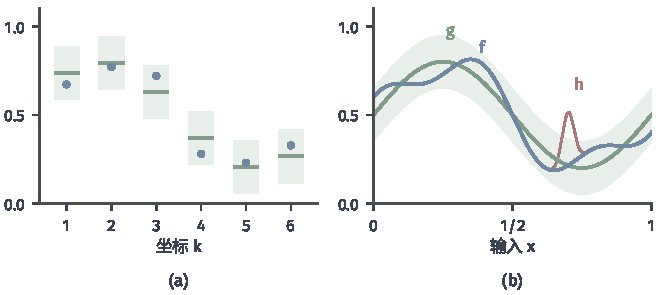
\includegraphics[width=112mm]{figures/04-spaces-measures-and-geometry/03-function-spaces/matplotlib/fcover-cube-tube/figure.pdf}
  \caption{一致距离的闭球。(a)绿色短线是代表$g$的六个坐标，绿色方框是各坐标$\pm\varepsilon$的范围（$\varepsilon=0.15$）；蓝点$f$的六个坐标都在方框内，表示$f$在这个闭球里。(b)同样的$g$与$f$画在全部输入上，方框连成管道。红色的$h$只在一小段上越出管道，一致距离仍把它判在球外。}
  \label{fig:fcover-cube-tube}
\end{BookInlineFigure}

图~\ref{fig:fcover-cube-tube}中，$f$在(a)的每个坐标上都落入方框，(b)中整条曲线留在管道里。一致距离只看最坏的坐标，$h$在别处都贴近$g$，在一小段上越出管道就算不合格。

类比也在这里显出困难。式~\eqref{eq:fcover-cube}的右端随$n$增大而趋于无穷，函数有无穷多个坐标，不能直接套用。真正的问题是：一类函数的无穷多个坐标，能否只用有限多个就决定到精度$\varepsilon$？

\paragraph{挑选近似与统一精度}

先看为单个函数找近似。给定$f\in C[0,1]$和$\varepsilon>0$，$f$在紧区间上一致连续，存在$m$，使$\lvert x-y\rvert\leq1/m$时$\lvert f(x)-f(y)\rvert\leq\varepsilon$。连接点$(j/m,f(j/m))$（$j=0,\ldots,m$）得到折线$g$。

设$x$在第$j$段上，局部位置为$t\in[0,1]$，则$g(x)$是两端值的凸组合，
\[
 f(x)-g(x)=(1-t)\Bigl(f(x)-f\bigl(\tfrac jm\bigr)\Bigr)+t\Bigl(f(x)-f\bigl(\tfrac{j+1}m\bigr)\Bigr).
\]
括号内的两项绝对值都不超过$\varepsilon$，所以$\lvert f(x)-g(x)\rvert\leq\varepsilon$。

这说明每个连续函数都有由$m+1$个数决定的近似，但$m$取决于$f$变化的快慢。为整类函数造表，要求的量词次序不同。两种说法分别是
\[
 \begin{gathered}
 \forall f\in\mathcal F,\ \exists\text{有限描述}\ g_f:\ \rho(f,g_f)\leq\varepsilon,\\
 \exists\text{有限集}\ V\subseteq E,\ \forall f\in\mathcal F,\ \exists v\in V:\ \rho(f,v)\leq\varepsilon .
 \end{gathered}
\]

第一种说法对$C[0,1]$总成立，第二种则要求一份预算服务全类。有限类总能造表，把成员全部列出即可。困难出在无限类上：若所需的节点数$m$随成员无限增大，就没有共同的预算，后面的鼓包正是这样。

\paragraph{距离的选择}

同一类函数在不同距离下可以有不同的答案。向量的情形已经能看出原因：两个$n$维向量只在一个坐标上相差$1$，最大分量差是$1$，平均分量差却只有$1/n$。

取$[0,1]$上的指示函数族$\mathcal F=\{\mathbf 1_{[0,t]}:0\leq t\leq1\}$，每个成员在某一点跳变。在$L^1[0,1]$中，两个成员之差的积分就是图~\ref{fig:fcover-indicator-distances}(b)中矩形的面积：
\[
 \lVert\mathbf 1_{[0,t]}-\mathbf 1_{[0,s]}\rVert_1=\lvert t-s\rvert .
\]
于是覆盖$\mathcal F$等同于用长度$2\varepsilon$的闭区间覆盖参数区间$[0,1]$。

\begin{BookInlineFigure}
  \centering
  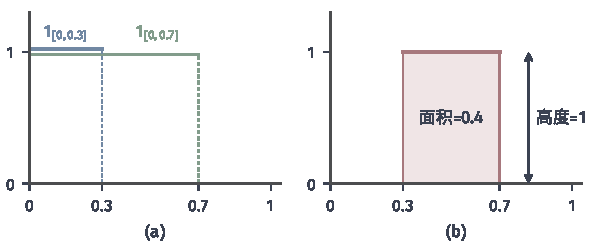
\includegraphics[width=100mm]{figures/04-spaces-measures-and-geometry/03-function-spaces/matplotlib/fcover-indicator-distances/figure.pdf}
  \caption{同一对函数的两种距离。(a)$\mathbf 1_{[0,0.3]}$（蓝）与$\mathbf 1_{[0,0.7]}$（绿）。(b)差的绝对值：$L^1$距离是红色矩形的面积$0.4$，一致距离是矩形的高度$1$。跳变点越靠近，面积越小，高度却始终是$1$。}
  \label{fig:fcover-indicator-distances}
\end{BookInlineFigure}

取$N=\lceil1/(2\varepsilon)\rceil$及$t_j=(2j-1)/(2N)$，每个$t$到最近的$t_j$不超过$1/(2N)\leq\varepsilon$，所以
\[
 N_{\mathcal F}(\varepsilon,\mathcal F)\leq\Bigl\lceil\frac1{2\varepsilon}\Bigr\rceil .
\]
例如$\varepsilon=0.1$时$N=5$，五个中心的跳变点是$0.1,0.3,0.5,0.7,0.9$。成员$\mathbf 1_{[0,0.62]}$对应最近的中心$t=0.7$，误差为$0.08$。

把同一族函数看作$[0,1]$上的有界函数，改用一致距离，情形就变了。$t\neq s$时两个指示函数在$t$与$s$之间相差$1$，所以两两距离都是$1$。半径$\varepsilon<1/2$的闭球若含其中两个，两者距离至多$2\varepsilon<1$，矛盾，因此每个球至多含一个成员。成员有不可数多个，覆盖数为$+\infty$。

积分距离允许误差集中在测度很小的集合上，一致距离不允许，两种答案的分界就在这里。

\paragraph{范数界不能保证有限覆盖}

最直接的约束是给出范数上界，即把$\mathcal F$放进一个闭球。这相当于把每个坐标限制在$[-M,M]$中，在有限维已足够，在无限维却不够。第~\ref{chap:functions-as-vectors}章用Riesz引理证明：任何无限维赋范空间的闭单位球中都有一列单位向量，两两距离至少为$1/2$。

半径$r<1/4$的闭球若含其中两个，两者距离至多$2r<1/2$，矛盾。所以无限维空间的闭单位球不能被半径小于$1/4$的有限个闭球覆盖。按比例缩放，半径$R$的闭球不能被半径小于$R/4$的有限个闭球覆盖。

在$C[0,1]$中可以把这一现象看得很具体。第~\ref{chap:functions-as-vectors}章的鼓包$\varphi_n$在$[\tfrac1{n+1},\tfrac1n]$的中点取$1$，在两端取$0$，区间外恒为$0$。不同鼓包的支撑至多相接于一点，所以$n\neq l$时
\[
 \lVert\varphi_n-\varphi_l\rVert_\infty=1 .
\]
全部$\varphi_n$都在闭单位球内，却没有半径小于$1/2$的有限覆盖。

\begin{BookInlineFigure}
  \centering
  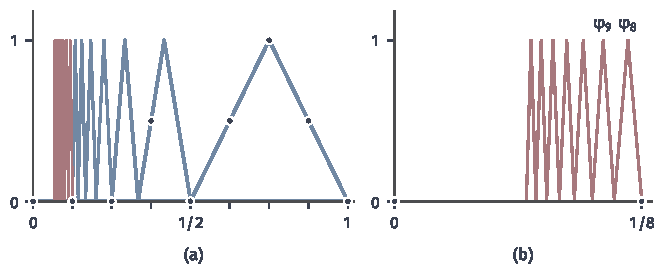
\includegraphics[width=112mm]{figures/04-spaces-measures-and-geometry/03-function-spaces/matplotlib/fcover-tents-on-grid/figure.pdf}
  \caption{固定网格看不见足够窄的鼓包。黑点是节点$j/8$。(a)蓝色为$\varphi_1,\ldots,\varphi_7$，红色为$\varphi_8,\ldots,\varphi_{14}$。(b)把$[0,1/8]$放大：红色鼓包的支撑全在两个节点之间，节点上的值都是$0$。}
  \label{fig:fcover-tents-on-grid}
\end{BookInlineFigure}

失败的原因可以从图~\ref{fig:fcover-tents-on-grid}读出来。固定一组节点$j/m$，当$n\geq m$时，$\varphi_n$的支撑含于$[0,1/m]$，内部没有节点，于是$\varphi_n$在每个节点上都为$0$。这些鼓包与零函数记录相同，一致距离却是$1$。

这也解释了斜率的作用。$\varphi_n$从$0$升到$1$只用了长度$1/(2n(n+1))$的区间，斜率为$2n(n+1)$，随$n$无界。用向量的语言说，每个鼓包占据一段自己的“坐标”，互相之间没有牵制，就像标准单位向量$e_n$。

要补上缺失的条件，有两个方向。第~\ref{sec:fcover-arzela-ascoli}节要求全类共用一个连续性尺度，让相邻坐标互相牵制；第~\ref{sec:fcover-finite-representations}节要求全类都贴近同一个有限维子空间，让靠后的坐标足够小。
